The ELPD and RMSE differences between models, relative to
the best model,
are shown in Figure \ref{fig:backtest-scores}.
When calculating ELPD, a small number of pointwise log densities 
showed very small, negative values, indicating poor predictions
on the out-of-sample data leading to numerical instability. 
We decided to remove any log predictive
densities for all models that had values $< -100$, which for a single
out-of-sample data point was particularly low, given that most
ELPD values for a single data point lie within [-5, 5]. This retained 99.7\%
of values for the PP results, 99.1\% of values for WC, 99.6\%
for CA, and 98.2\% for OO. The full log densities are given in the
supplementary materials, as well as results for different levels
of filtering.

For ELPD, at least one of the
hidden Markov model variants out-performed
the latent change-point and 
two-step models, on average, 
apart from ELPD values for the PP
lines of business where the latent change-point
performed marginally better than the nearest
HMM model. The standard errors around the ELPD
values, however, indicated that all the models
often performed within 2 standard errors from each other,
apart from the OO line of business where the HMM models
performed noticeably better.
For all lines of business, one of the HMM 
models clearly out-performed the latent change-point
and two-step models in RMSE.
Overall, the HMM-$\nu$ model attained
75\% of the best average ELPD scores, and 50\%
of the best average RMSE scores, meaning that
allowing for tail processes to revert
to the body is an important feature in making
future predictions.
Evaluating the predictions at the 10th
development period
out-of-sample values only, to mirror
the estimation of ultimate loss,
mirrored the results in Figure
\ref{fig:backtest-scores} apart from some
minor changes in ranks of the HMM
models (full results are supplied
in the code repository).
The performance results also indicated
that the latent change-point model
was close to, but still out-performed,
on average, the two-step in both ELPD and RMSE.


\begin{figure}
    \centering
    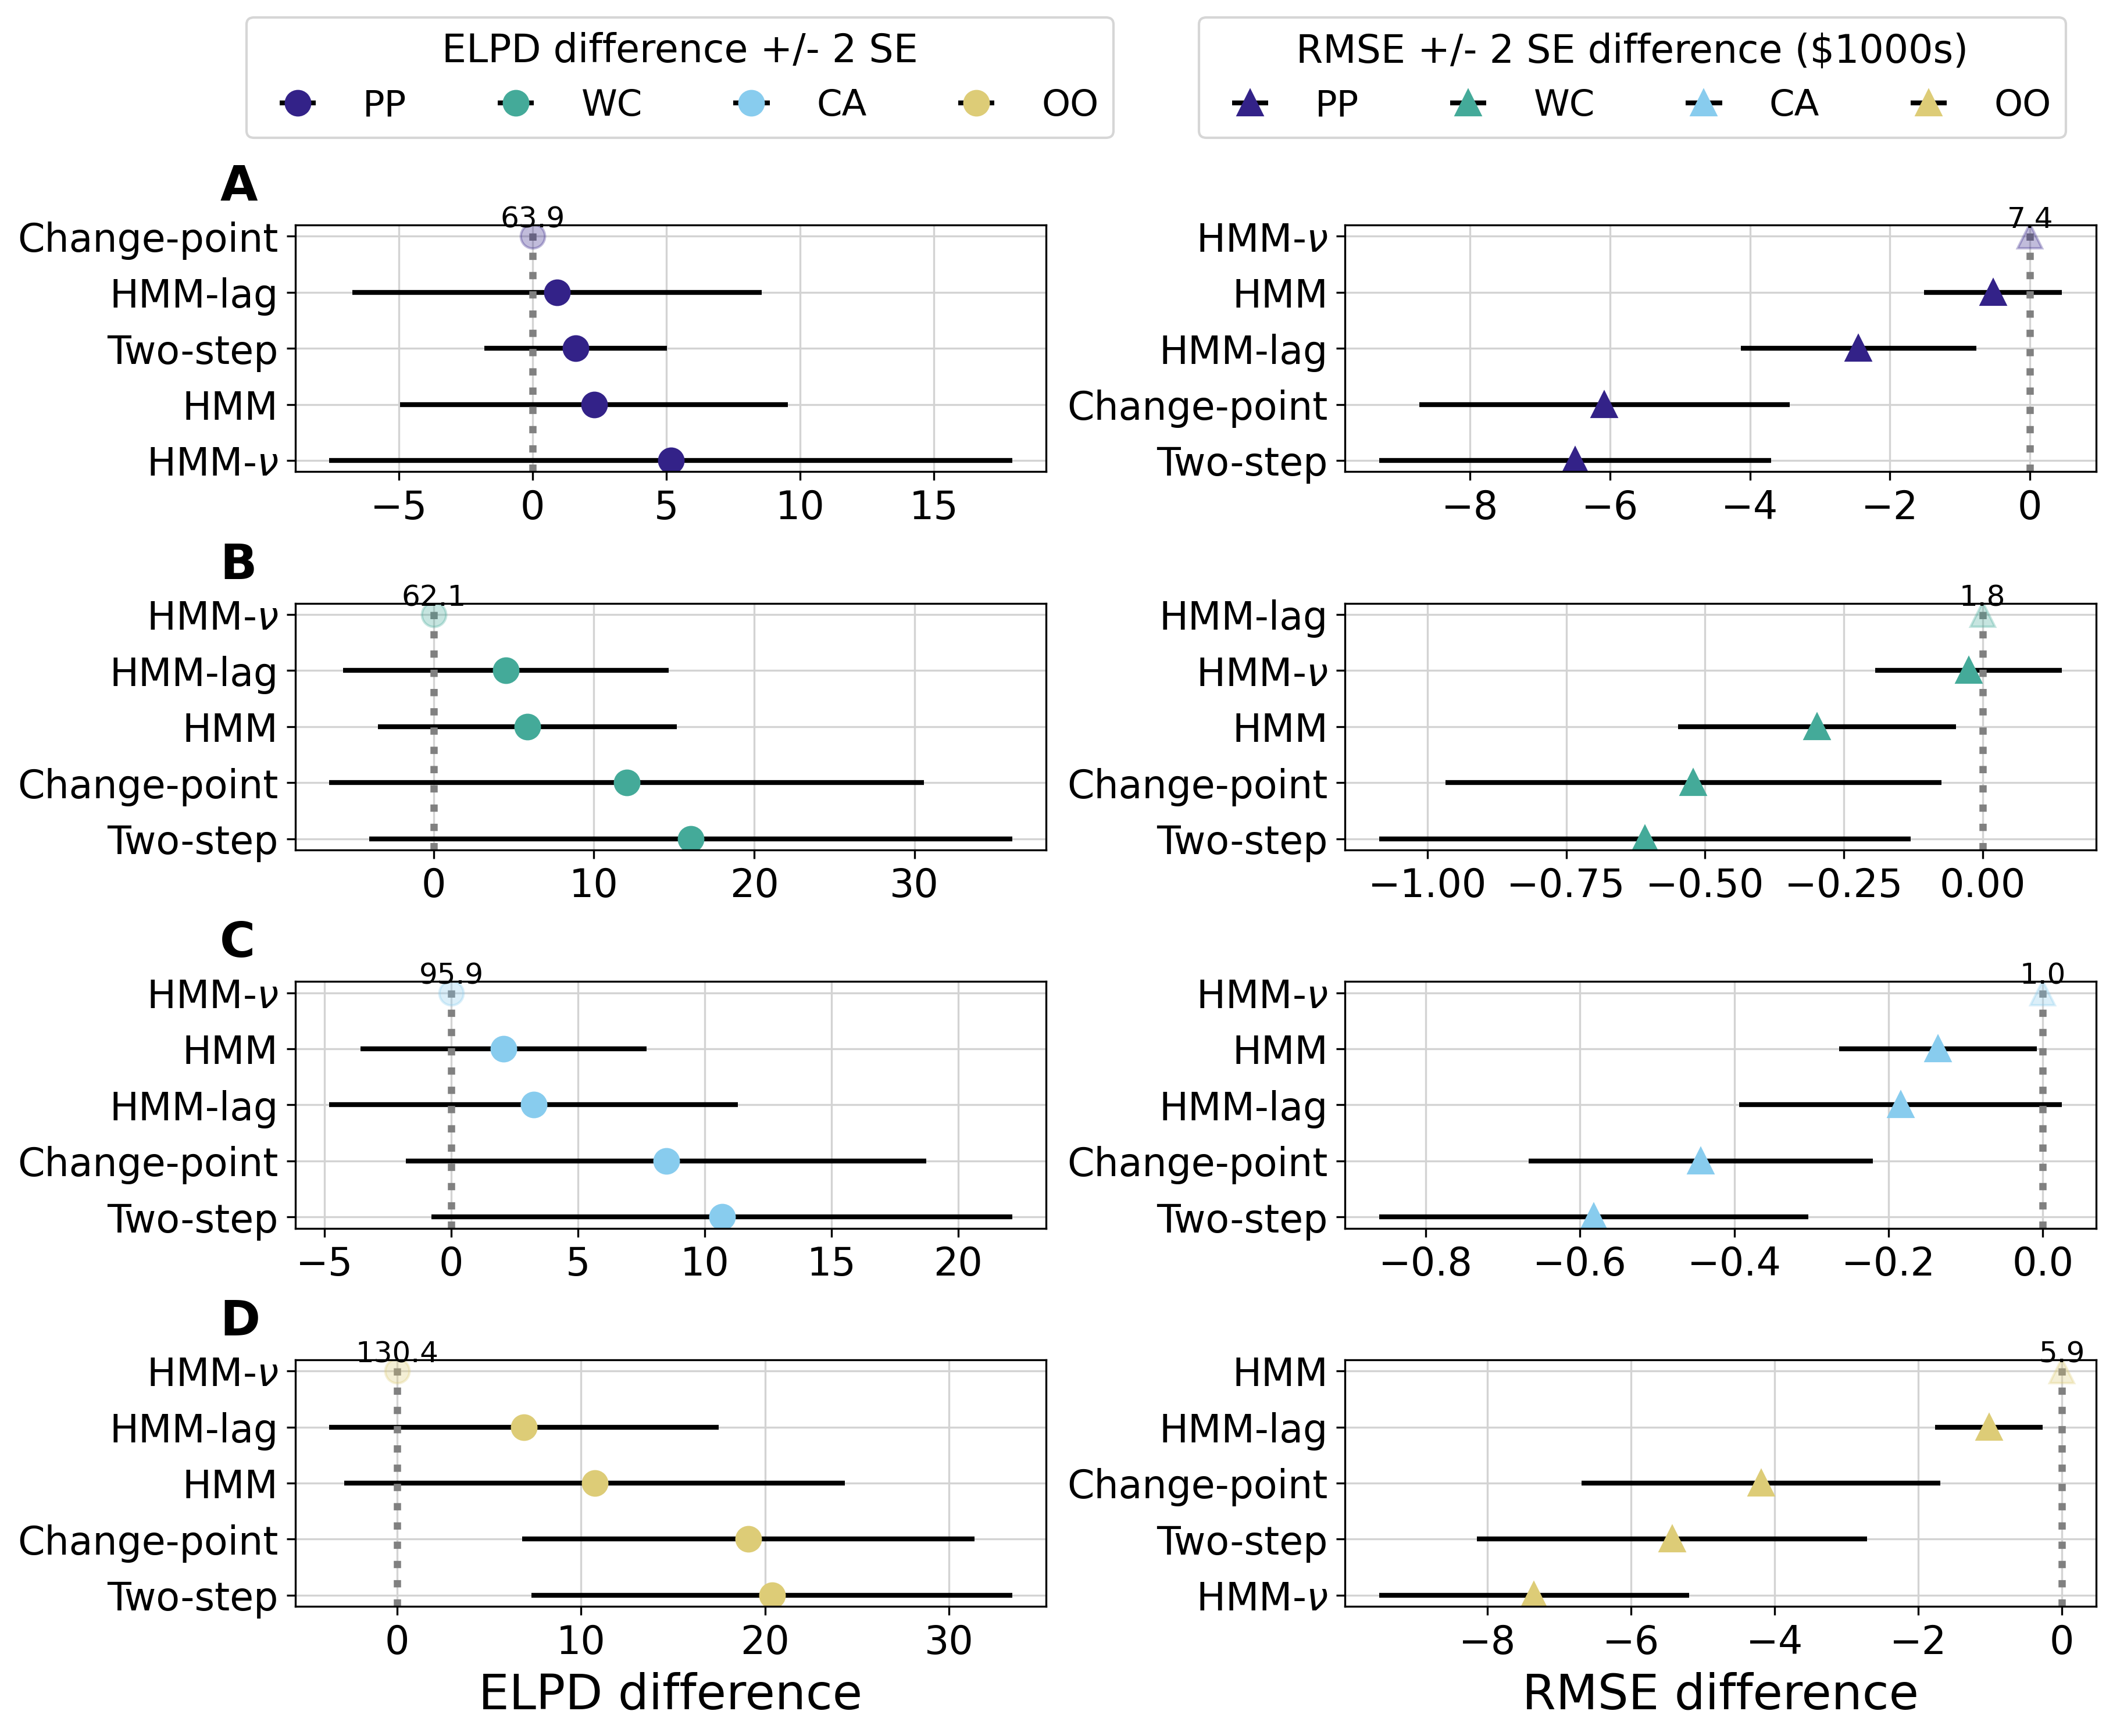
\includegraphics[scale=0.45]{\figures/scores.png}
    \caption{
        The ELPD (left column) and RMSE (in thousands of dollars; right column)
		differences (+/- 2 standard errors; SE) in order of performance
        for each model and line of business for the industry
        triangles. Rows A through D enumerate results
        for line of business separately.
        The best-performing model is shown at the top of each
        panel, with the absolute ELPD or RMSE value displayed above.
        Positive ELPD differences with an uncertainty interval that does not
        cross zero indicates a credible difference at the 95\% level
        in favour of the top model.
        Negative RMSE differences with an uncertainty interval
        that does not cross zero indicates a credible difference
        in favour of the top model.
    }
	\label{fig:backtest-scores}
\end{figure}

Model calibration histograms (Figure \ref{fig:percentiles})
indicated that both the hidden Markov models
and two-step approaches typically have predictions that
are too uncertain, indicated by the inverted-U shaped
histograms. In WC, the hidden Markov models had the most
uniform percentiles, whereas the two-step approach
showed signs of both under- and over-estimation.

\begin{figure}
    \centering
    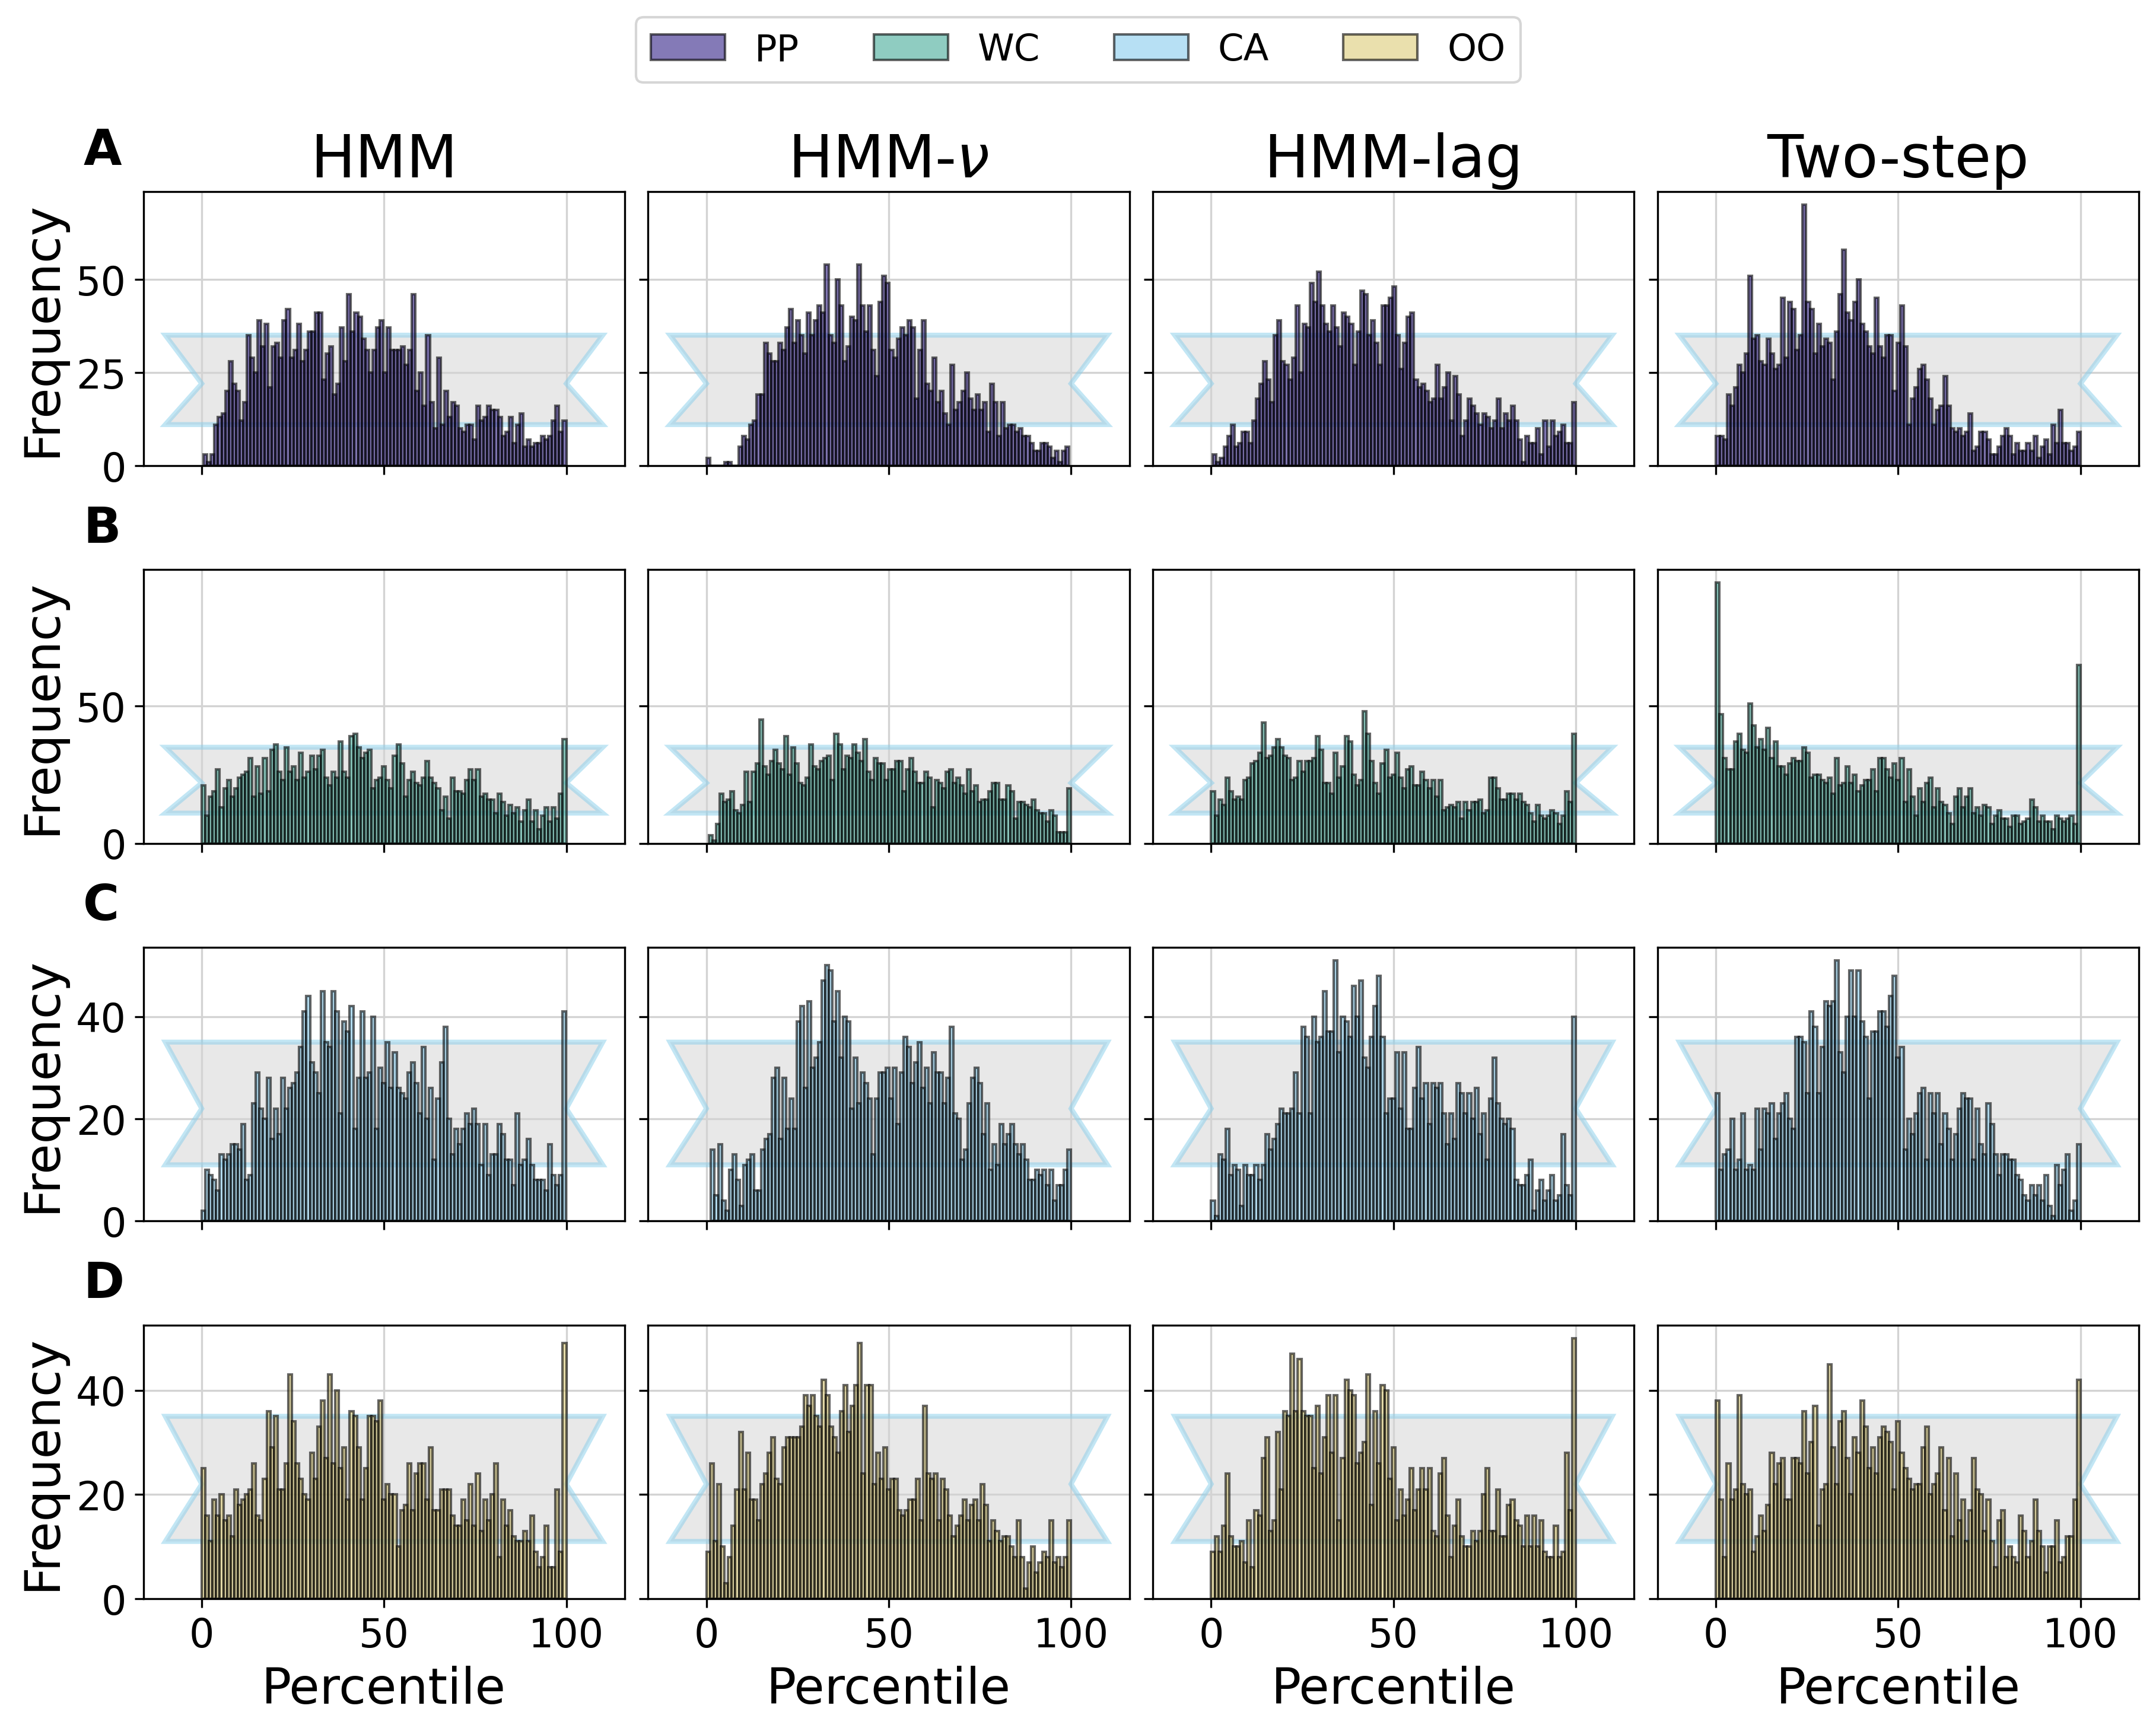
\includegraphics[scale=0.45]{\figures/calibration.png}
    \caption{
        Percentiles of the true left-out values on the posterior distributions
        for each model and line of business (panels A through D) in the industry triangles.
        Grey shaded regions provide the 99\% intervals of a discrete uniform
        distribution, for reference.
        Right-skewed histograms indicate under-estimation,
        left-skewed histograms indicate over-estimation,
        and inverted-U histograms indicate predictions that
        are uncertain.
    }
    \label{fig:percentiles}
\end{figure}

The hidden Markov model variants had different
implications for body-to-tail switch-over points
depending on the particular line of business
(Figure \ref{fig:zstars}).
The PP and CA lines showed, in general,
the quickest development to the tail
state, at development period 2 for the HMM
and HMM-$\nu$ models, and by development
period 3 for most accident periods for the
HMM-lag model. In contrast, WC stayed
longest in the body state, followed by
OO, and both WC and OO lines demonstrated
relatively equitable probabilities of being
in the body and tail at later development
periods. This is particularly noticeable for
the HMM-$\nu$ model, where the chance
of returning to the body from tail process
was allowed.

\begin{figure}
    \centering
    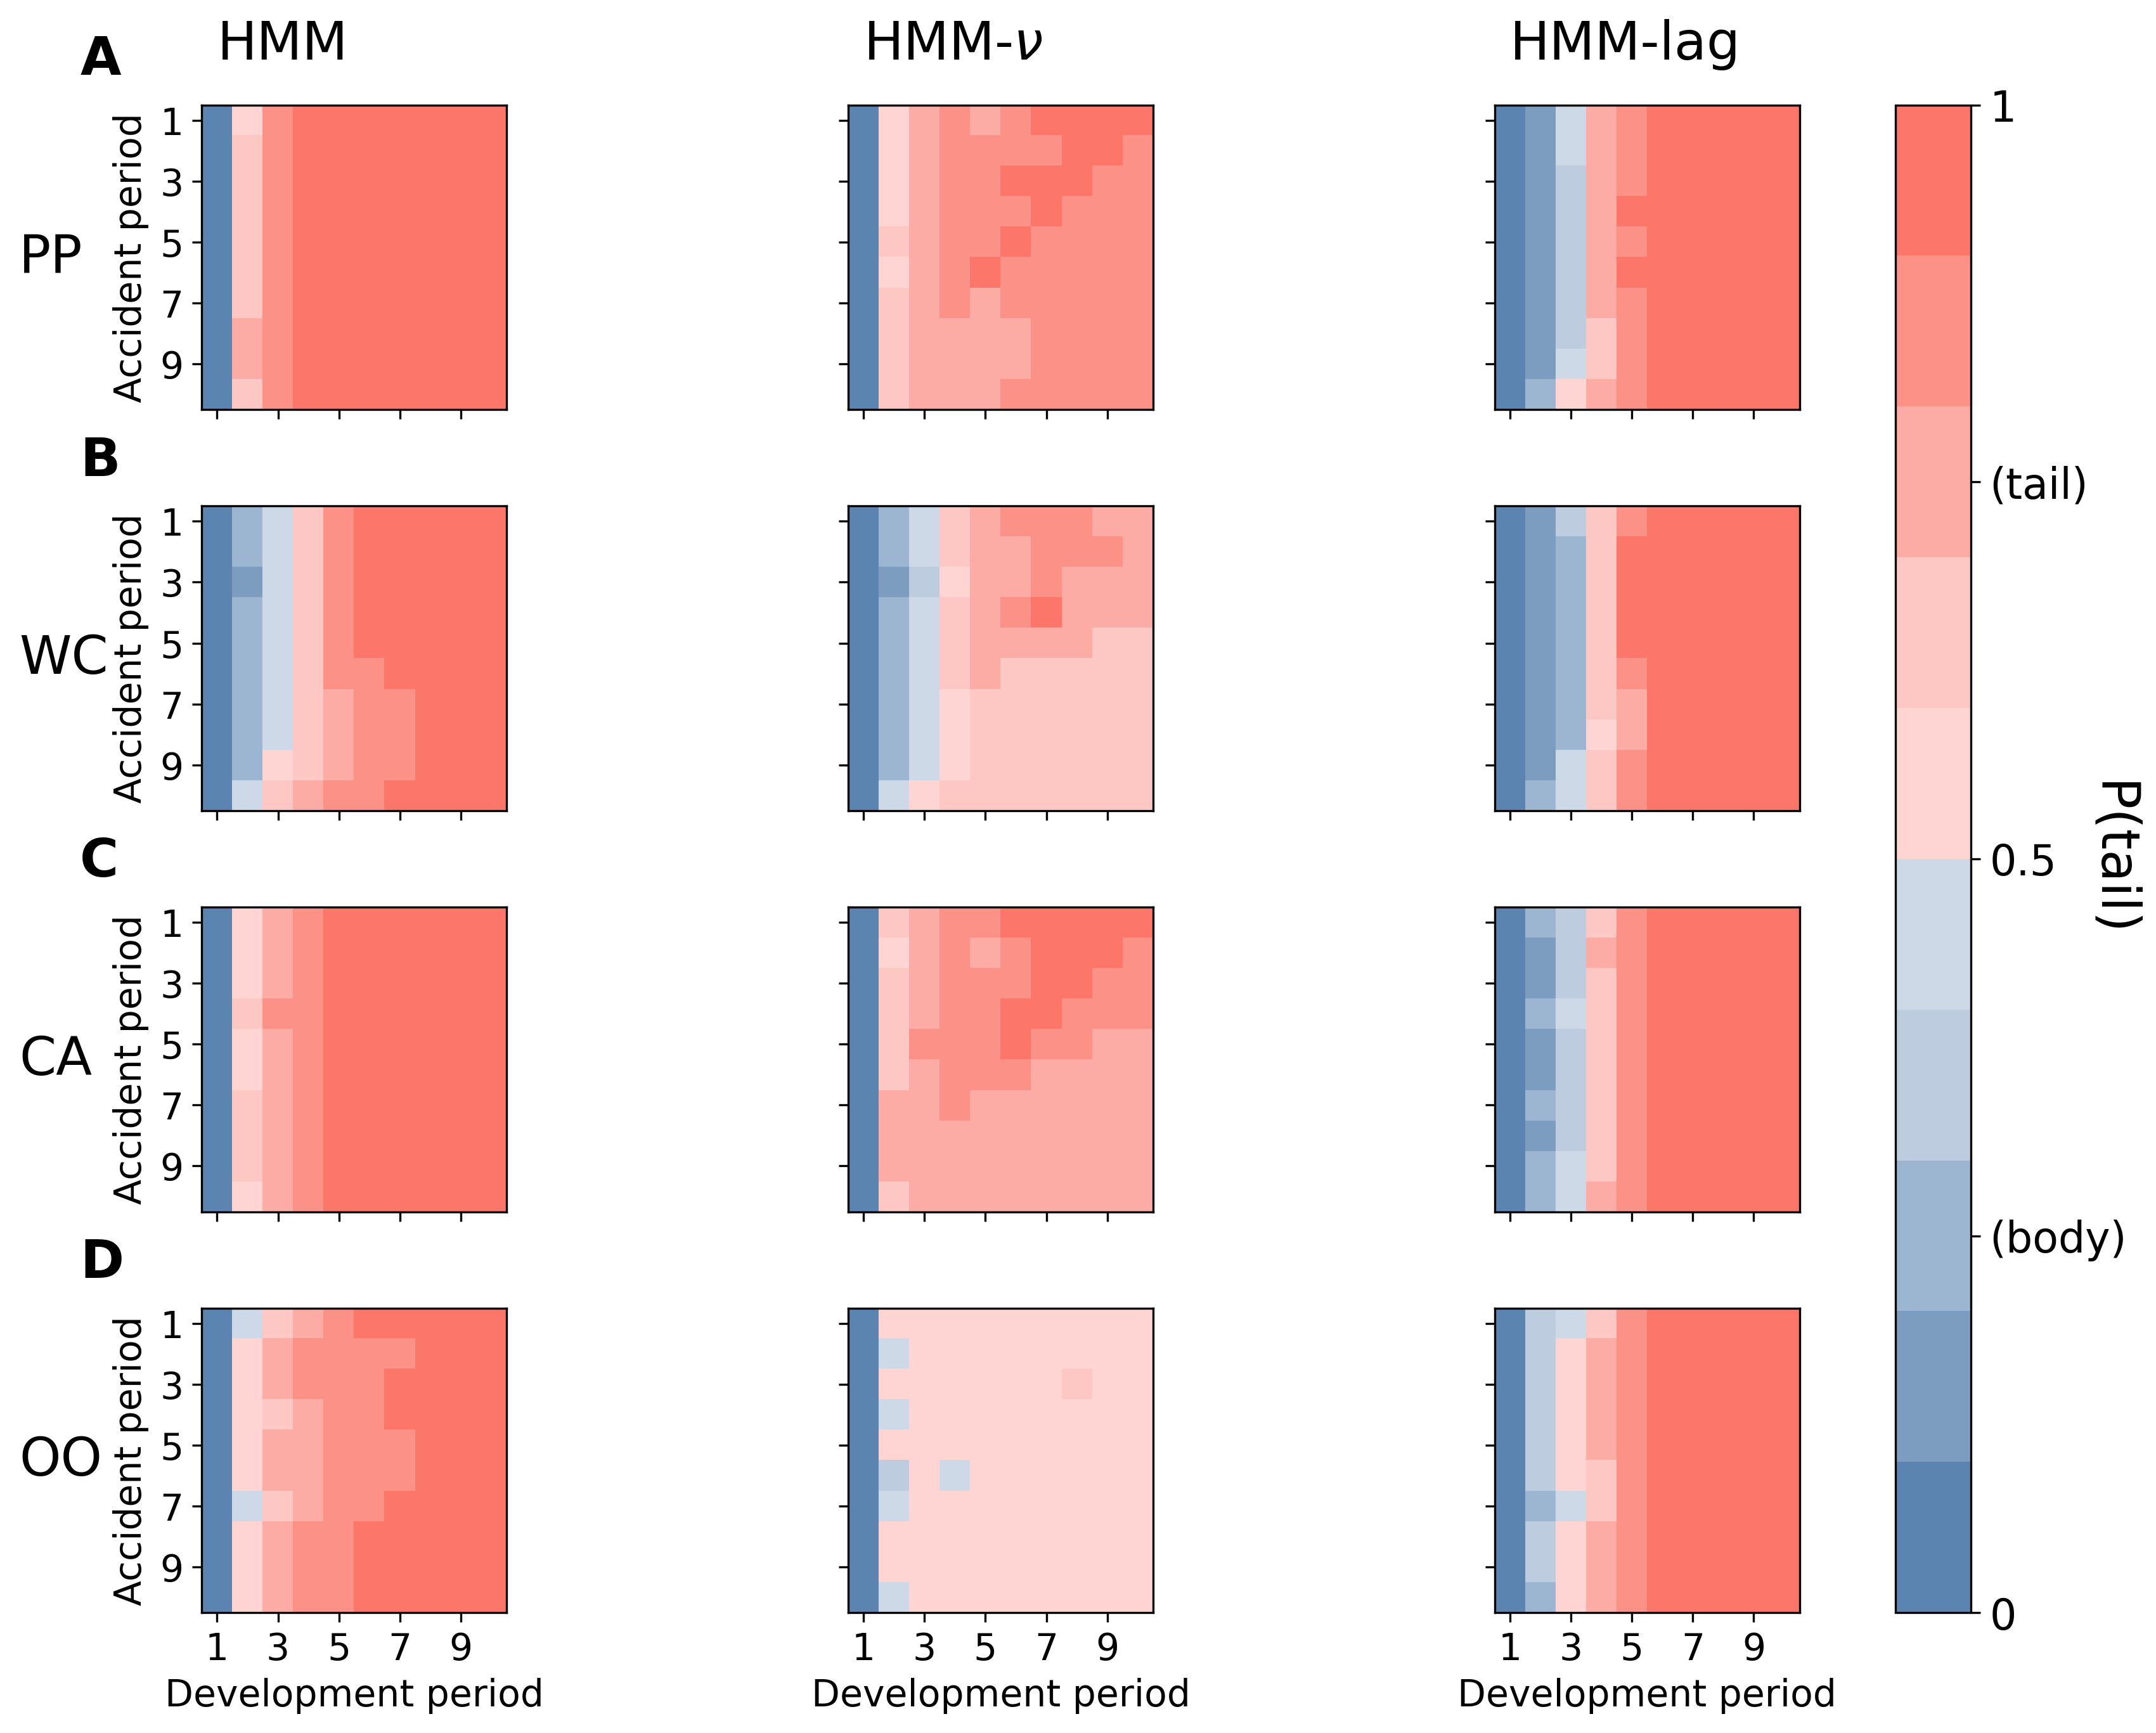
\includegraphics[scale=0.45]{\figures/z_stars.png}
    \caption{
        The average probability of being in the tail process
        for each hidden Markov model parameterization (columns)
        and line of business (rows A-D) across triangles
        in the industry data.
        Probabilities $\leq 0.5$ are coloured
        in blue whereas probabilities $> 0.5$
        are coloured in orange. More faded squares
        indicating smaller probabilities of being
        in body and tail processes, respectively.
    }
    \label{fig:zstars}
\end{figure}

For the five literature triangles, the lack
of hold-out data meant that the uncertainties
around the ELPD and RMSE differences
indicated more equal model performance
(Figure \ref{fig:literature}).
The average ELPD
differences indicated that one of the hidden
Markov models or the latent change-point
model performed better than the
two-step approach.
However, the two-step model
performed on-par with the change-point
and hidden Markov models in terms of RMSE,
and clearly performed best in RMSE
for the \cite{verrall2015} triangle
because of the triangle's relative smooth, 
gradual dynamics.
The manual selection of $\tau$
for the two-step process often
closely aligned with the 
posterior distribution of most
plausible $\tau$ values estimated by the latent
change-point model.

\begin{figure}
    \centering
    \hspace{-1em}
    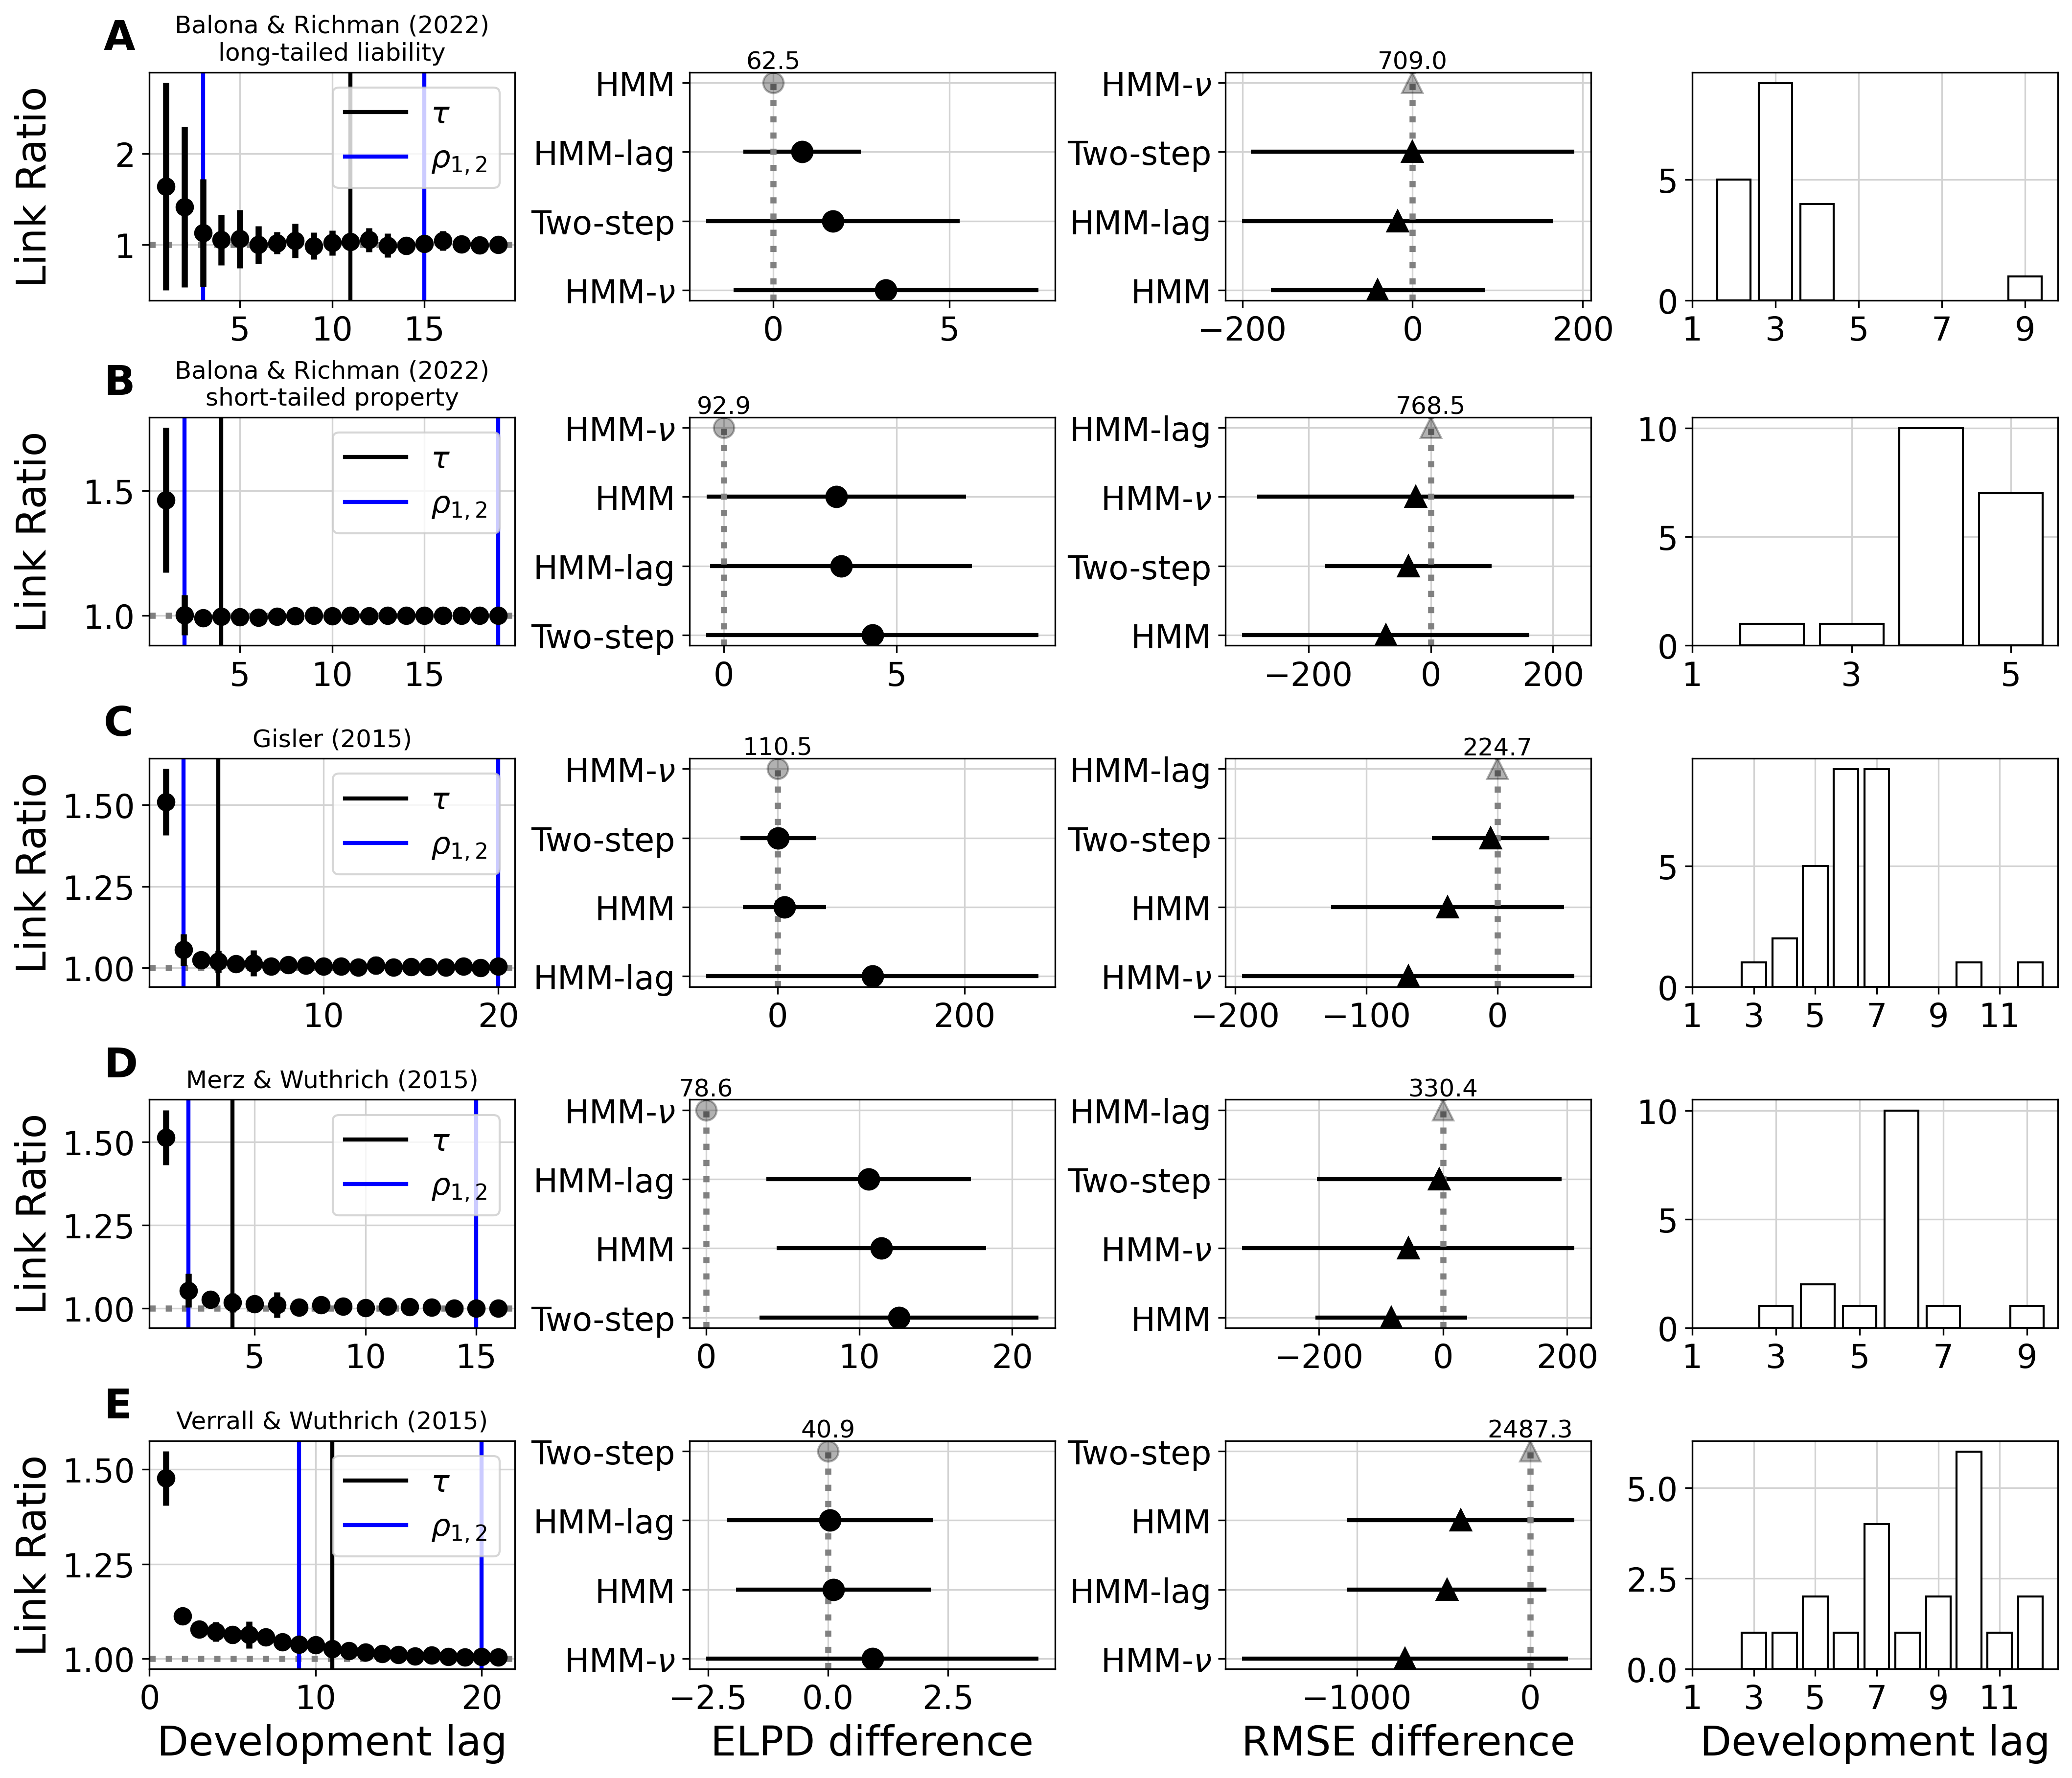
\includegraphics[scale=0.4]{\figures/literature.png}
    \caption{
        Model results on the five literature triangles
        (rows A - D). The first
        column shows the mean (+/- 2 standard deviations)
        of the empirical link ratios in the triangles.
        The black and blue vertical lines indicate $\tau$
        and $\bm{\rho} = \rho_{1:2}$, the tail start
        and generalised Bondy model training windows,
        respectively (see model definitions, above).
        The second column presents the distribution
        of $\tau$ values from the latent change-point,
        for comparison to the two-step manual values
        shown in the first column.
        The third and final columns show the
        ELPD and RMSE differences (+/- 2 SE) from the best
        performing model (top model in each panel), calculated
        from predictions on the latest diagonal of
        data (out-of-sample) in the loss triangles.
        The absolute ELPD and RMSE of the best-performing
        models are shown above the top model, for reference.
    }
	\label{fig:literature}
\end{figure}

